\documentclass[oneside,openany,headings=optiontotoc,11pt,numbers=noenddot]{scrreprt}

\usepackage[a4paper]{geometry}
\usepackage[utf8]{inputenc}
\usepackage[T1]{fontenc}
\usepackage{lmodern}
\usepackage[ngerman]{babel}
\usepackage{ngerman}

\usepackage[onehalfspacing]{setspace}

\usepackage{fancyhdr}
\usepackage{fancybox}

\usepackage{rotating}
\usepackage{varwidth}

%Struktogramme
\usepackage[german,curves]{struktex}

\usepackage{pdflscape}
\usepackage{changepage}
\usepackage{graphicx}
\usepackage[bottom]{footmisc}
\usepackage{transparent}
\usepackage{graphbox}
\graphicspath{
	{Pics/PDFs/}
	{Pics/JPGs/}
	{Pics/PNGs/}
}
\usepackage{caption}
\usepackage{wrapfig}
\usepackage{marginnote}
\usepackage{tabularx}
\usepackage{dashrule}
\usepackage{soulutf8}
\usepackage{hhline}
%arydshln suppresses vertical lines in table
%\usepackage{arydshln}
\usepackage{multirow}
\usepackage{enumerate}
\usepackage[hidelinks]{hyperref}
\usepackage{listings}

\usepackage[table]{xcolor}
\usepackage{array}
\usepackage{enumitem,amssymb,amsmath}
\usepackage{interval}
\usepackage{cancel}
\usepackage{stmaryrd}
\usepackage{wasysym}
\usepackage{polynom}
\usepackage{diagbox}
\usepackage{dashrule}
\usepackage{framed}
\usepackage{mdframed}
\usepackage{karnaugh-map}
\usepackage{pdfpages}

\usepackage{blindtext}

\usepackage{eso-pic}

\usepackage{amssymb}
\usepackage{eurosym}

\usepackage[pages=some]{background}
\pagestyle{headings}
\renewcommand{\headrulewidth}{0.2pt}
\renewcommand{\footrulewidth}{0.2pt}
\newcommand*{\underdownarrow}[2]{\ensuremath{\underset{\overset{\Big\downarrow}{#2}}{#1}}}
\setlength{\fboxsep}{5pt}
\newcommand{\explainBelow}[3]{\underbrace{#1}_{\parbox{\widthof{#3}}{\footnotesize\raggedright #2}}}
\newcommand{\explainAbove}[3]{\overbrace{#1}^{\parbox{\widthof{#3}}{\footnotesize\raggedright #2}}}
\newcommand\footnoteref[1]{\protected@xdef\@thefnmark{\ref{#1}}\@footnotemark}


% Codestyle defined
\definecolor{codegreen}{rgb}{0,0.6,0}
\definecolor{codegray}{rgb}{0.5,0.5,0.5}
\definecolor{codepurple}{rgb}{0.58,0,0.82}
\definecolor{backcolour}{rgb}{0.95,0.95,0.92}
\definecolor{deepgreen}{rgb}{0,0.5,0}
\definecolor{darkblue}{rgb}{0,0,0.65}
\definecolor{mauve}{rgb}{0.40, 0.19,0.28}
\colorlet{exceptioncolour}{yellow!50!red}
\colorlet{commandcolour}{blue!60!black}
\colorlet{numpycolour}{blue!60!green}
\colorlet{specmethodcolour}{violet}

%Neue Spaltendefinition
\newcolumntype{L}[1]{>{\raggedright\let\newline\\\arraybackslash\hspace{0pt}}m{#1}}
\newcolumntype{M}{>{\centering\arraybackslash}X}
\newcommand{\cmnt}[1]{\ignorespaces}
%Textausrichtung ändern
\newcommand\tabrotate[1]{\rotatebox{90}{\raggedright#1\hspace{\tabcolsep}}}

%Intervall-Konfig
\intervalconfig {
	soft open fences
}

%Bash
\lstdefinestyle{BashInputStyle}{
	language=bash,
	basicstyle=\small\sffamily,
	backgroundcolor=\color{backcolour},
	columns=fullflexible,
	backgroundcolor=\color{backcolour},
	breaklines=true,
}
%Java
\lstdefinestyle{JavaInputStyle}{
	language=Java,
	backgroundcolor=\color{backcolour},
	aboveskip=1mm,
	belowskip=1mm,
	showstringspaces=false,
	columns=flexible,
	basicstyle={\footnotesize\ttfamily},
	numberstyle={\tiny},
	numbers=none,
	keywordstyle=\color{purple},,
	commentstyle=\color{deepgreen},
	stringstyle=\color{blue},
	emph={out},
	emphstyle=\color{darkblue},
	emph={[2]rand},
	emphstyle=[2]\color{specmethodcolour},
	breaklines=true,
	breakatwhitespace=true,
	tabsize=2,
}
%Python
\lstdefinestyle{PythonInputStyle}{
	language=Python,
	alsoletter={1234567890},
	aboveskip=1ex,
	basicstyle=\footnotesize,
	breaklines=true,
	breakatwhitespace= true,
	backgroundcolor=\color{backcolour},
	commentstyle=\color{red},
	otherkeywords={\ , \}, \{, \&,\|},
	emph={and,break,class,continue,def,yield,del,elif,else,%
		except,exec,finally,for,from,global,if,import,in,%
		lambda,not,or,pass,print,raise,return,try,while,assert},
	emphstyle=\color{exceptioncolour},
	emph={[2]True,False,None,min},
	emphstyle=[2]\color{specmethodcolour},
	emph={[3]object,type,isinstance,copy,deepcopy,zip,enumerate,reversed,list,len,dict,tuple,xrange,append,execfile,real,imag,reduce,str,repr},
	emphstyle=[3]\color{commandcolour},
	emph={[4]ode, fsolve, sqrt, exp, sin, cos, arccos, pi,  array, norm, solve, dot, arange, , isscalar, max, sum, flatten, shape, reshape, find, any, all, abs, plot, linspace, legend, quad, polyval,polyfit, hstack, concatenate,vstack,column_stack,empty,zeros,ones,rand,vander,grid,pcolor,eig,eigs,eigvals,svd,qr,tan,det,logspace,roll,mean,cumsum,cumprod,diff,vectorize,lstsq,cla,eye,xlabel,ylabel,squeeze},
	emphstyle=[4]\color{numpycolour},
	emph={[5]__init__,__add__,__mul__,__div__,__sub__,__call__,__getitem__,__setitem__,__eq__,__ne__,__nonzero__,__rmul__,__radd__,__repr__,__str__,__get__,__truediv__,__pow__,__name__,__future__,__all__},
	emphstyle=[5]\color{specmethodcolour},
	emph={[6]assert,range,yield},
	emphstyle=[6]\color{specmethodcolour}\bfseries,
	emph={[7]Exception,NameError,IndexError,SyntaxError,TypeError,ValueError,OverflowError,ZeroDivisionError,KeyboardInterrupt},
	emphstyle=[7]\color{specmethodcolour}\bfseries,
	emph={[8]taster,send,sendMail,capture,check,noMsg,go,move,switch,humTem,ventilate,buzz},
	emphstyle=[8]\color{blue},
	keywordstyle=\color{blue}\bfseries,
	rulecolor=\color{black!40},
	showstringspaces=false,
	stringstyle=\color{deepgreen}
}

\lstset{literate=%
	{Ö}{{\"O}}1
	{Ä}{{\"A}}1
	{Ü}{{\"U}}1
	{ß}{{\ss}}1
	{ü}{{\"u}}1
	{ä}{{\"a}}1
	{ö}{{\"o}}1
}

% Neue Klassenarbeits-Umgebung
\newenvironment{worksheet}[3]
% Begin-Bereich
{
	\newpage
	\sffamily
	\setcounter{page}{1}
	\ClearShipoutPicture
	\AddToShipoutPicture{
		\put(55,761){{
				\mbox{\parbox{385\unitlength}{\tiny \color{codegray}BBS I Mainz, #1 \newline #2
						\newline #3
					}
				}
			}
		}
		\put(455,761){{
				\mbox{\hspace{0.3cm}
\includegraphics[width=0.2\textwidth]{../../logo.pdf}}
			}
		}
	}
}
% End-Bereich
{
	\clearpage
	\ClearShipoutPicture
}

\geometry{left=2.50cm,right=2.50cm,top=3.00cm,bottom=1.00cm,includeheadfoot}

\begin{document}
	\begin{worksheet}{Höhere Berufsfachschule IT-Systeme}{Grundstufe - Mathematik}{Wochenplan Grundlagen}
		\noindent
		\begin{tabularx}{\textwidth}{XXl}
			Wochenplan Nr.: \underline{    3    } & & Zeitraum: \underline{27.08 - 02.09}
		\end{tabularx}
	
		\begin{framed}
			\noindent
			\textbf{Montag:}  Bestimmen Sie die Lösungsmenge der Gleichungen und Ungleichungen:\\
			\begin{tabularx}{\textwidth}{ll}
				\\
				(a) \(\frac{1}{2}x + \frac{3}{2} = 1 + \frac{5}{2}x\) & |\(-\frac{1}{2}x; -1\)\\
				\(\frac{1}{2} = 2x\) & |\(:2\)\\
				\(\frac{1}{4} = x\)\\
				\(\Rightarrow \mathbb{L} = \{\frac{1}{4}\}\)\\
				\\
				(b) \(-\frac{2}{9}x - \frac{1}{4} = -\frac{3}{2}-\frac{1}{6}x\) & |\(+\frac{2}{9}x; +\frac{3}{2}\)\\
				\(\frac{5}{4} = \frac{1}{18}x\) & |\(\cdot{}18\)\\
				\(\frac{45}{2} = x\)\\
				\(\Rightarrow \mathbb{L} = \{\frac{45}{2}\}\)\\
				\\
				(c) \(x-12 = 3-4x\) & |\(+4x; +12\)\\
				\(5x = 15\) & |\(:5\)\\
				\(x = 3\)\\
				\(\Rightarrow \mathbb{L}=\{3\}\)\\
				\\
				(d) \((13a+12)(12a-13) = (12a+3)(13a+9)\) & | AM\\
				\(156a^2 \underbrace{-25a}_{-169a + 144a} -156 = 156a^2 + \underbrace{147a}_{108a +39a} +27\) & |\(-156a^2; +25a; -27\)\\
				\(-183 = 172a\) & |\(:172\)\\
				\(-\frac{183}{172} = a\)\\
				\(\Rightarrow \mathbb{L} = \{-\frac{183}{172}\}\)\\
				\\
				(e) \(-\frac{3}{5}x-\frac{5}{2} > -\frac{1}{2}x + \frac{2}{5}\) & |\(+\frac{3}{5}x; -\frac{2}{5}\)\\
				\(-\frac{29}{10} > \frac{1}{10}x\) & |\(\cdot{}10\)\\
				\(-29 > x\)\\
				\(\Rightarrow \mathbb{L} = \{x < -29\}\)\\
				\\
				(f) \(\frac{1}{5}x-\frac{1}{2}>1+\frac{2}{5}x\) & |\(-\frac{1}{5}x; -1\)\\
				\(-\frac{3}{2} > \frac{1}{5}x\) & |\(\cdot{}5\)\\
				\(-\frac{15}{2}> x\)\\
				\(\Rightarrow \mathbb{L} = \{x < -\frac{15}{2}\}\)
			\end{tabularx}
		\end{framed}
		\newpage
		\begin{framed}
			\noindent
			\textbf{Dienstag:} Berechnen Sie die Lösung der nachfolgenden Bruchrechnungen:\\
			\begin{tabularx}{\textwidth}{X}
				\\
				(a) \(\frac{1}{a-3} - \frac{1}{a+3} = \frac{a+3}{(a-3)(a+3)}- \frac{a-3}{(a-3)(a+3)} = \frac{a+3 - (a-3)}{(a-3)(a+3)} = \frac{6}{(a-3)(a+3)}\)\\
				\\
				(b) \(\frac{a+b}{a-3}-\frac{a-b}{a+3} = \frac{(a+b)(a+3)}{(a-3)(a+3)}- \frac{(a-b)(a-3)}{(a-3)(a+3)} = \frac{(a^2-3a+ab+3b) - (a^2 -3a -ab +3b)}{(a-3)(a+3)}\)\\
				\\
				\(= \frac{a^2-3a+ab+3b - a^2 +3a +ab -3b}{(a-3)(a+3)} = \frac{2ab}{(a-3)(a+3)}\)\\
				\\
				(c) \(\frac{a+1}{a-2}- \frac{a-1}{a+3} = \frac{(a+1)(a+3)}{(a-2)(a+3)}- \frac{(a-1)(a-2)}{(a-2)(a+3)} = \frac{(a^2 + 4a + 3) - (a^2 +a -6)}{(a-2)(a+3)}\)\\
				\\
				\(= \frac{a^2 + 4a + 3 - a^2 -a +6}{(a-2)(a+3)} = \frac{3a +6}{(a-2)(a+3)}\)\\
				\\
				(d) \(\frac{2a+1}{a-b} + \frac{a-2}{a+2} = \frac{(2a+1)(a+2)}{(a-b)(a+2)}- \frac{(a-2)(a-b)}{(a-b)(a+2)} = \frac{(2a^2+5a+3) - (a^2 -ab -2a +2b)}{(a-b)(a+2)}\)\\
				\\
				\(\frac{2a^2+5a+3 - a^2 +ab +2a -2b)}{(a-b)(a+2)} = \frac{a^2 + 7a +ab -2b +3}{(a-b)(a+2)}\)
			\end{tabularx}
		\end{framed}
		\begin{framed}
			\noindent
			\textbf{Mittwoch:} Stellen Sie eine Wertetabelle, von \(f(x)\) auf. Beginnen Sie mit \(x = -2\) und geben die Werte bis \(x = 6\) an. Schrittweite 1.\\
			(a) \(f(x) = 12x^2 - 4x\)\\
			\begin{tabularx}{\textwidth}{l|M|M|M|M|M|M|M|M|M}
				x & \(-2\) & \(-1\) & \(0\) & \(1\) & \(2\) & \(3\) & \(4\) & \(5\) & \(6\)\\
				\hline
				y & \(56\) & \(16\) & \(0\) & \(8\) & \(40\) & \(96\) & \(176\) & \(280\) & \(408\)\\ 
			\end{tabularx}\\
			\par\noindent
			(b) \(f(x) = -3x + 5\)\\
			\begin{tabularx}{\textwidth}{l|M|M|M|M|M|M|M|M|M}
				x & \(-2\) & \(-1\) & \(0\) & \(1\) & \(2\) & \(3\) & \(4\) & \(5\) & \(6\)\\
				\hline
				y & \(11\) & \(8\) & \(5\) & \(2\) & \(-1\) & \(-4\) & \(-7\) & \(-10\) & \(-13\)\\  
			\end{tabularx}\\
			\par\noindent
			(c) \(f(x) = 12x^2-21x+13\)\\
			\begin{tabularx}{\textwidth}{l|M|M|M|M|M|M|M|M|M}
				x & \(-2\) & \(-1\) & \(0\) & \(1\) & \(2\) & \(3\) & \(4\) & \(5\) & \(6\)\\
				\hline
				y & \(103\) & \(46\) & \(13\) & \(4\) & \(19\) & \(58\) & \(121\) & \(208\) & \(219\)\\ 
			\end{tabularx}\\
			\par\noindent
			(d) \(f(x) = x^3 - 2x^2 + x - 1\)\\
			\begin{tabularx}{\textwidth}{l|M|M|M|M|M|M|M|M|M}
				x & \(-2\) & \(-1\) & \(0\) & \(1\) & \(2\) & \(3\) & \(4\) & \(5\) & \(6\)\\
				\hline
				y & \(-19\) & \(-5\) & \(-1\) & \(-1\) & \(1\) & \(11\) & \(35\) & \(79\) & \(149\)\\ 
			\end{tabularx}\\
		\end{framed}
		\newpage
		\begin{framed}
			\noindent
			\textbf{Donnerstag:} Bestimmen Sie die Wertetabelle zu \(f(x)\) und übertragen Sie die berechneten Punkte in ein Koordinatensystem:\\
			(a) \(f(x) = 3x-5\)\\
			\begin{tabularx}{\textwidth}{l|M|M|M|M|M|M|M|M|M}
				x & \(-2\) & \(-1\) & \(0\) & \(1\) & \(2\) & \(3\) & \(4\) & \(5\) & \(6\)\\
				\hline
				y & \(-11\) & \(-8\) & \(-5\) & \(-2\) & \(1\) & \(4\) & \(7\) & \(10\) & \(13\)\\ 
			\end{tabularx}\\
			\par\noindent
			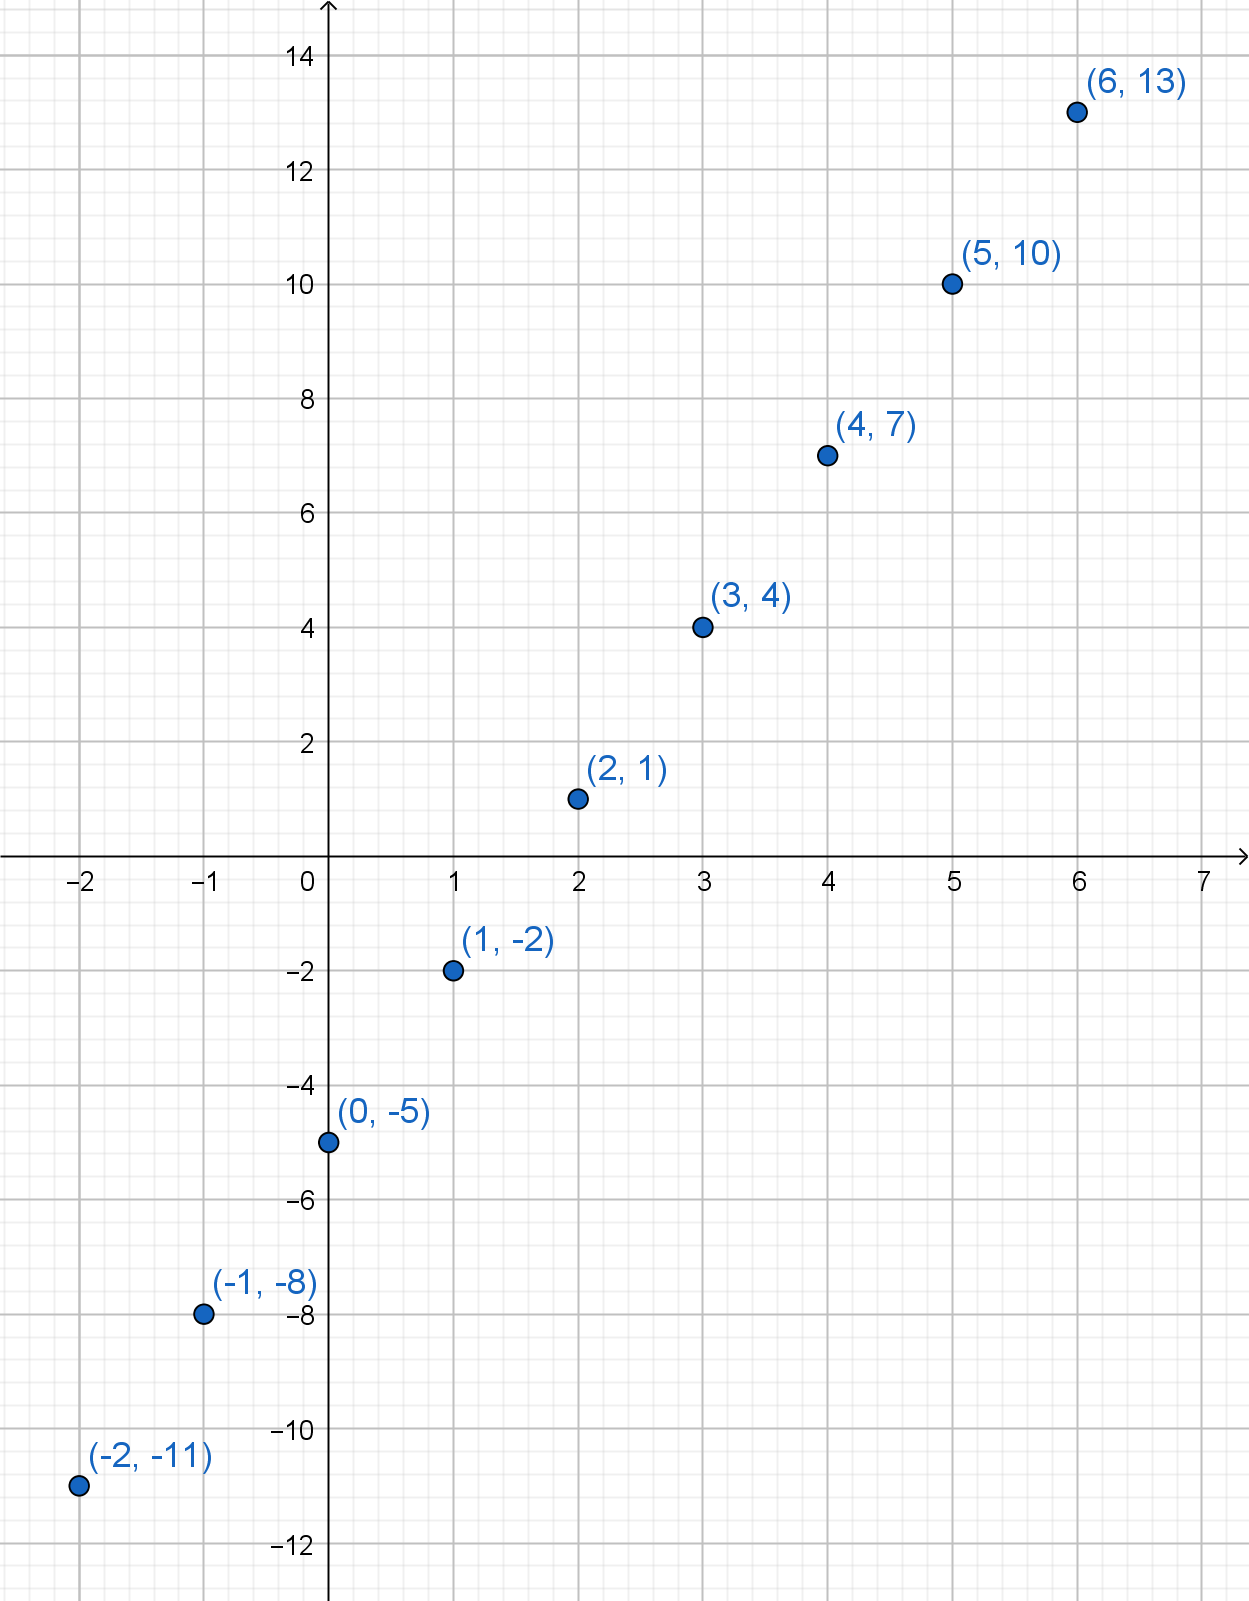
\includegraphics[width=0.95\textwidth]{../99_Bilder/WP3Doa.png}\\
			(b) \(f(x) = \frac{1}{2}x^2 + 2 \)\\
			\begin{tabularx}{\textwidth}{l|M|M|M|M|M|M|M|M|M}
				x & \(-2\) & \(-1\) & \(0\) & \(1\) & \(2\) & \(3\) & \(4\) & \(5\) & \(6\)\\
				\hline
				y & \(4\) & \(2,5\) & \(2\) & \(2,5\) & \(4\) & \(6,5\) & \(10\) & \(14,5\) & \(20\)\\  
			\end{tabularx}\\
			\par\bigskip\noindent
			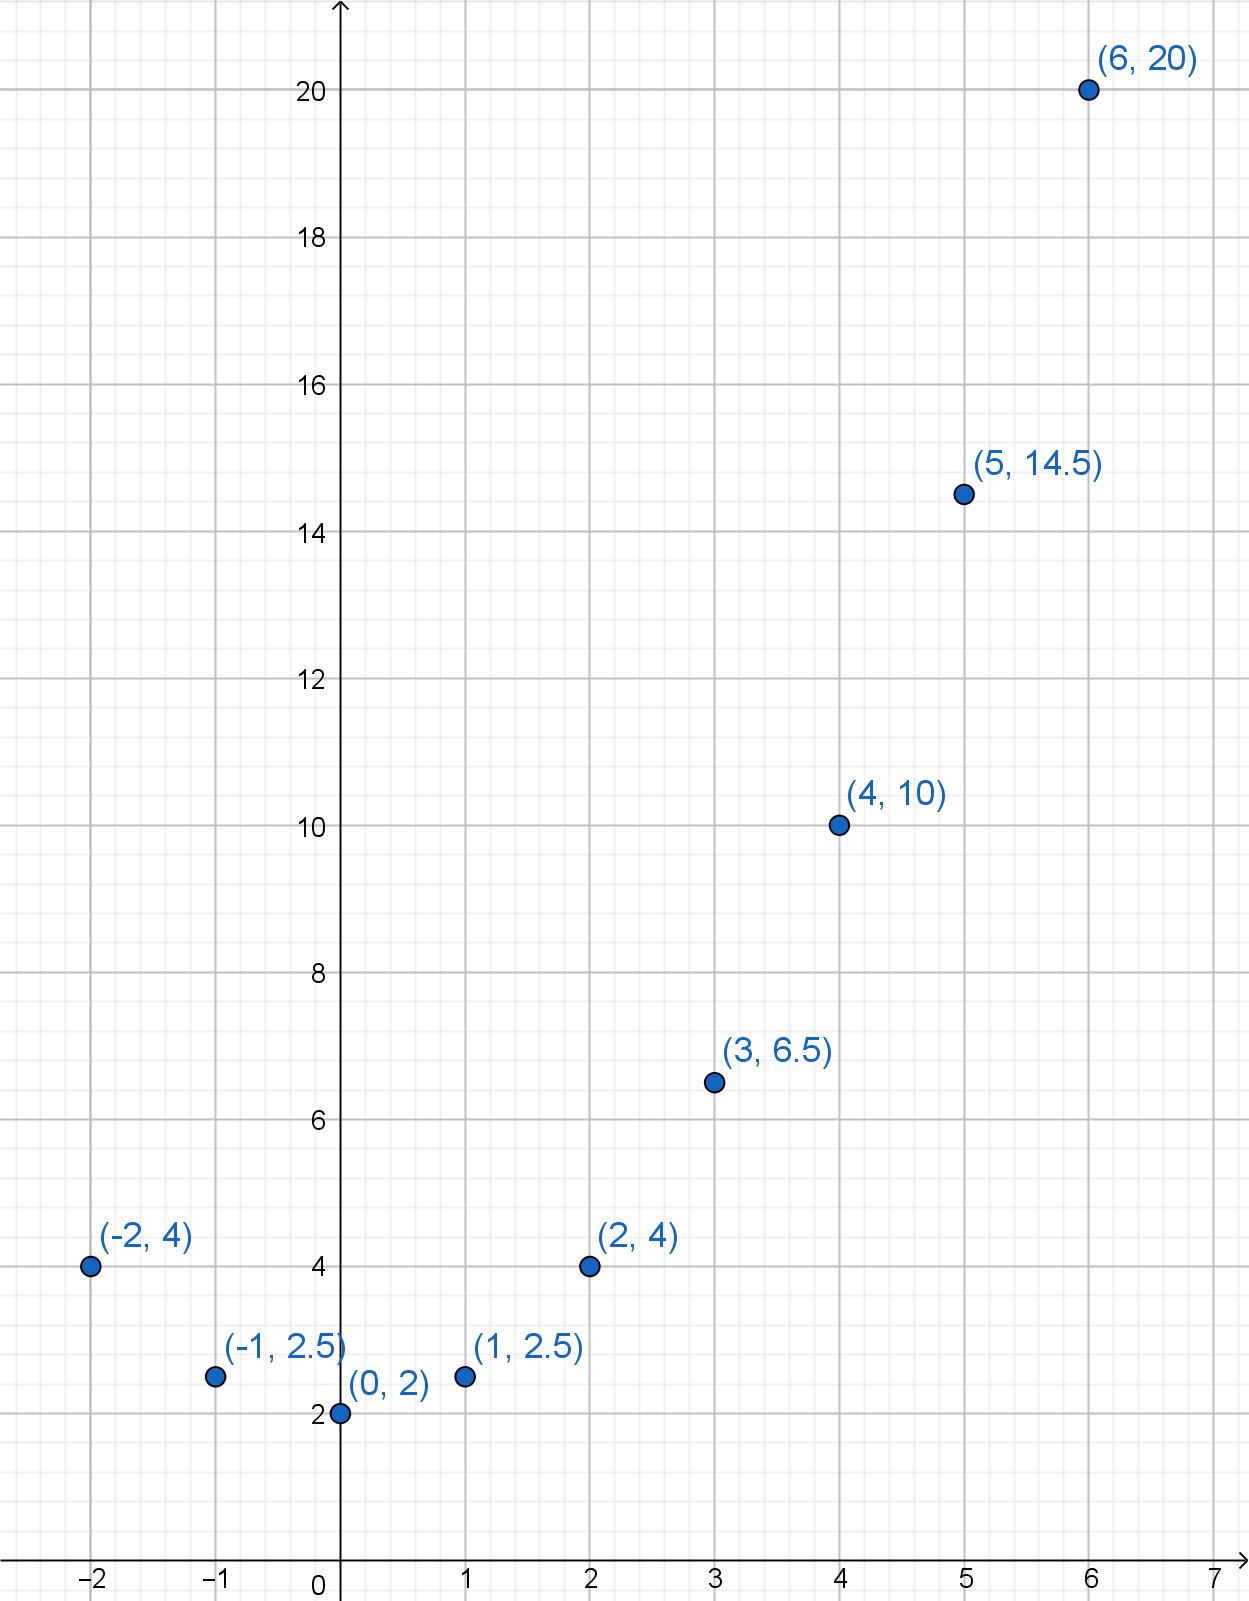
\includegraphics[width=0.95\textwidth]{../99_Bilder/WP3Dob.png}\\
			\par\noindent
			(c) \(f(x) = \frac{1}{2}x +1\)\\
			\begin{tabularx}{\textwidth}{l|M|M|M|M|M|M|M|M|M}
				x & \(-2\) & \(-1\) & \(0\) & \(1\) & \(2\) & \(3\) & \(4\) & \(5\) & \(6\)\\
				\hline
				y & \(0\) & \(0,5\) & \(1\) & \(1,5\) & \(2\) & \(2,5\) & \(3\) & \(3,5\) & \(4\)\\ 
			\end{tabularx}\\
			\par\noindent
			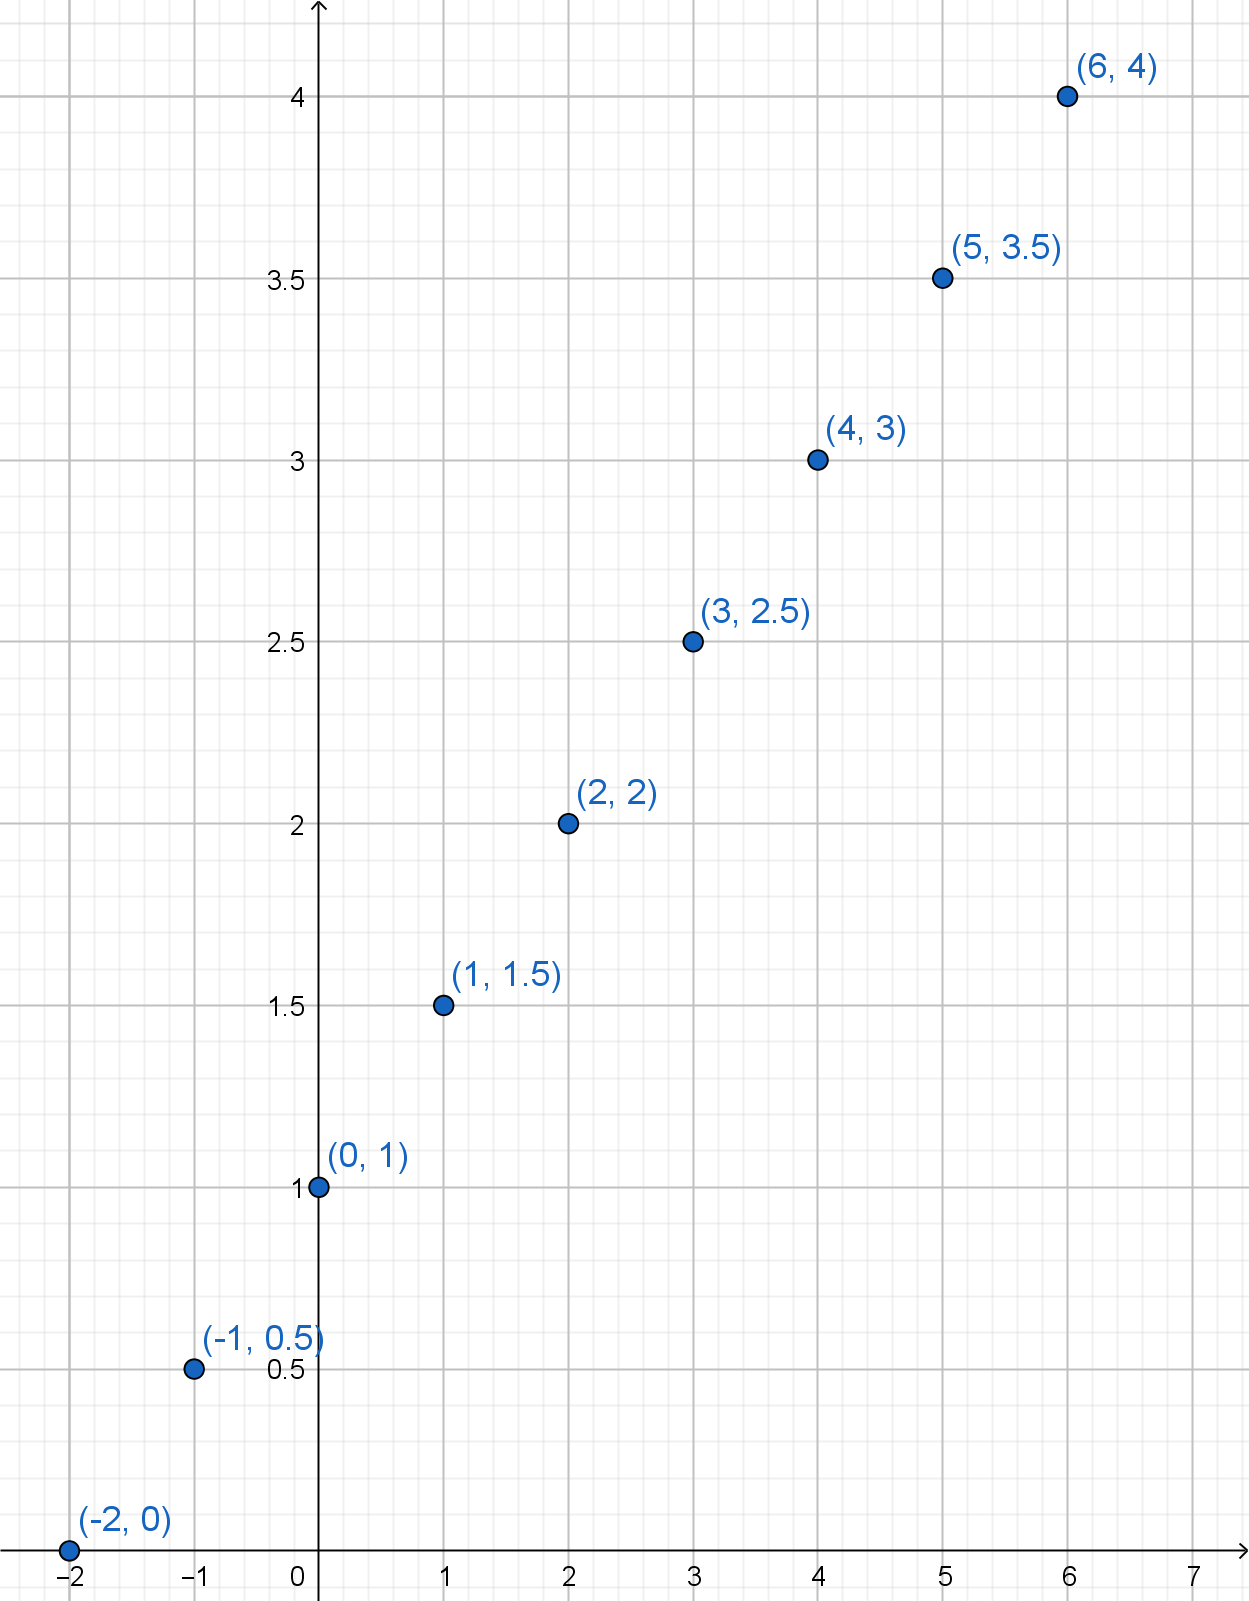
\includegraphics[width=0.95\textwidth]{../99_Bilder/WP3Doc.png}\\
			\par\bigskip\noindent
			(d) \(f(x) = -3x-1\)\\
			\begin{tabularx}{\textwidth}{l|M|M|M|M|M|M|M|M|M}
				x & \(-2\) & \(-1\) & \(0\) & \(1\) & \(2\) & \(3\) & \(4\) & \(5\) & \(6\)\\
				\hline
				y & \(5\) & \(2\) & \(-1\) & \(-4\) & \(-7\) & \(-10\) & \(-13\) & \(-16\) & \(-19\)\\ 
			\end{tabularx}\\
			\par\noindent
			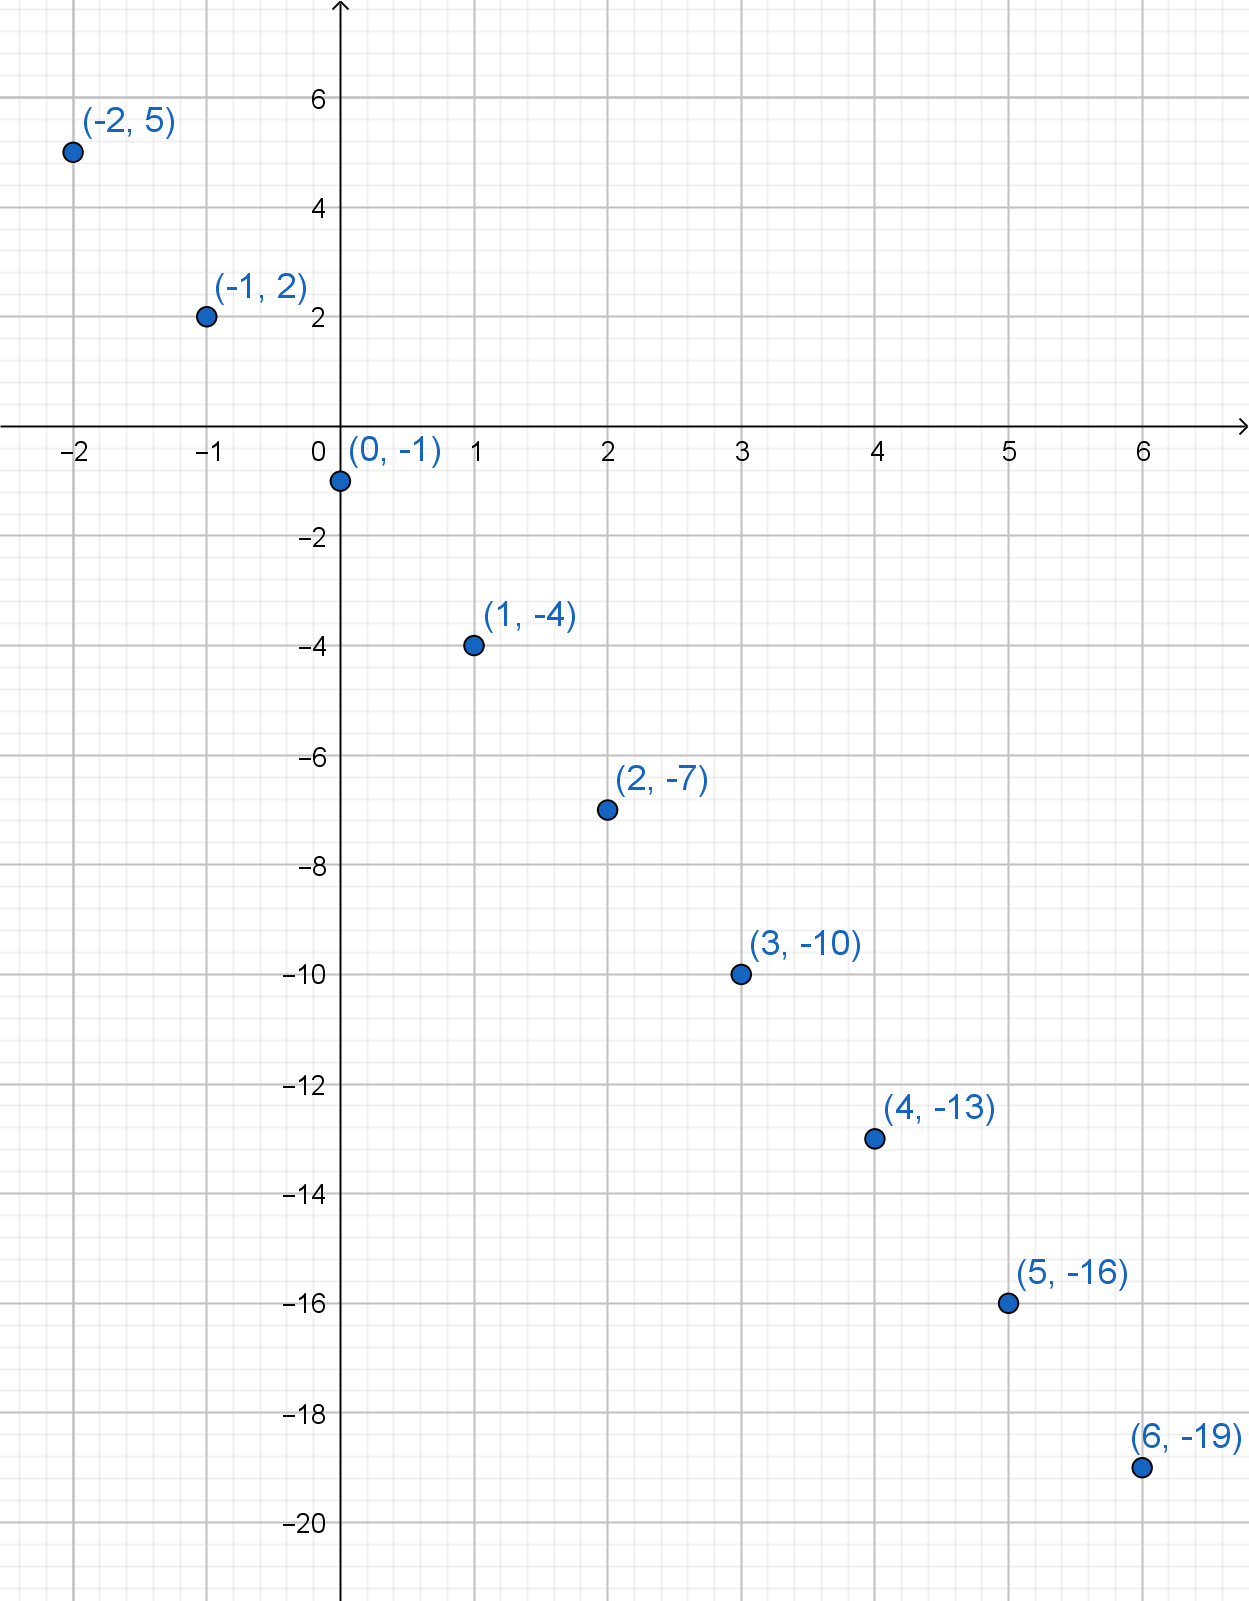
\includegraphics[width=0.95\textwidth]{../99_Bilder/WP3Dod.png}\\
			\par\noindent
		\end{framed}
		\newpage
		\begin{framed}
			\noindent
			\textbf{Freitag:} Berechnen Sie den Wert der Funktion an der Stelle \(x = 3\).\\
			\par\noindent
			\begin{tabularx}{\textwidth}{X|X}
				(a) \(f(x) = -\frac{1}{3}x + 3\) & (b) \(f(x) = 3x^2 - 3x + 12\)\\
				& \\
				\(f(3) = -\frac{1}{3}\cdot{}3 + 3 = 2\) & \(f(3) = 3\cdot{}3^2 - 3\cdot{}3 + 12 = 30\)\\
				& \\
				\hline
				& \\
				(c) \(f(x) = (x+2)^2\) & (d) \(f(x) = \frac{17}{4}x^3 - 3x^2 + x - 14\)\\
				& \\
				\(f(3) = (3+2)^2 = 5^2 = 25\) & \(f(x) = \frac{17}{4}\cdot{}3^3 - 3\cdot{}3^2 + 3 - 14 = \frac{307}{4}\)
			\end{tabularx}
		\end{framed}
	\end{worksheet}
\end{document}